% LLNCS macro package for Springer Computer Science proceedings;
% Version 2.20 of 2017/10/04
%
\documentclass[runningheads]{llncs}
%
\usepackage{graphicx}
% Used for displaying a sample figure. If possible, figure files should
% be included in EPS format.
%
% If you use the hyperref package, please uncomment the following line
% to display URLs in blue roman font according to Springer's eBook style:
% \renewcommand\UrlFont{\color{blue}\rmfamily}

% My packages
\usepackage{orcidlink} % Orcid links
\newcommand\Mark[1]{\textsuperscript#1}

\usepackage{amssymb} % \square command
% Footnotes inside tables
\usepackage{footnote}
\usepackage{csquotes} % enquote command
\usepackage{glossaries} % Glossary
\usepackage{threeparttable} % Tables with notes
\makesavenoteenv{tabular}
\makesavenoteenv{table}
% Acronyms
\newacronym{bpmn}{BPMN}{Business Process Modeling Notation}
\newacronym{gt}{GT}{Graph Transformation}
\newacronym{mt}{MT}{Model Transformation}
\newacronym{hot}{HOT}{Higher-Order model Transformation}
% Fix underscore in dois
\usepackage[strings]{underscore}

\begin{document}
%
\title{Formalization and analysis of BPMN using graph transformation systems}
%
%\titlerunning{Abbreviated paper title}
% If the paper title is too long for the running head, you can set
% an abbreviated paper title here
%
\author{Tim Kr\"{a}uter\inst{1}\orcidlink{0000-0003-1795-0611} \and
Adrian Rutle\inst{1}\orcidlink{0000-0002-4158-1644} \and
Harald K\"{o}nig\inst{2,1}\orcidlink{0000-0001-6304-6311} \and
Yngve Lamo\inst{1}\orcidlink{0000-0001-9196-1779}}
%
\authorrunning{T. Kräuter et al.}
% First names are abbreviated in the running head.
% If there are more than two authors, 'et al.' is used.
%
\institute{Western Norway University of Applied Sciences, Bergen, Norway 
\email{tkra@hvl.no, aru@hvl.no, yla@hvl.no} \and
University of Applied Sciences, FHDW, Hanover, Germany\\
\email{harald.koenig@fhdw.de}}
%
\maketitle              % typeset the header of the contribution
%
\begin{abstract}
The Business Process Modeling Notation (BPMN) is a widely used standard notation for defining intra- and inter-organizational workflows.
However, the informal description of the BPMN execution semantics leads to different interpretations of BPMN elements and difficulties in checking behavioral properties.
In this paper, we propose a formalization of the execution semantics of BPMN that, compared to existing approaches, covers more BPMN elements while faciliating property checking.
Our approach is based on a higher-order transformation from BPMN models to graph transformation systems.
As proof of concept, we have implemented our approach in an open-source web-based tool.

\keywords{BPMN \and Model transformation \and Graph transformation \and Model checking \and Formalization}
\end{abstract}

\section{Introduction}
In today's fast-paced business environment, organisations with complex workflows require a powerful means to accurately map, analyse, and optimize their processes. 
\gls*{bpmn} \cite{objectmanagementgroupBusinessProcessModel2013} is widely used standard to define these workflows.
However, the informal description of the \gls*{bpmn} execution semantics leads to different interpretations of \gls*{bpmn} elements and difficulties in checking behavioral properties \cite{corradiniFormalApproachAnalysis2021}.
Formalizing \gls*{bpmn} would reduce the cost of business process automation drastically by facilitating the detection of errors and optimization potentials in process models already during design time. 
To this end, we propose a formalization that covers most of the \gls*{bpmn} elements used in practice and supports checking behavioral properties.

In this paper, we consider two fundamental concepts when formalizing the execution semantics of \gls*{bpmn}.
First, \textit{state structure}, i.e., how models are represented during execution.
The state structure corresponds to the type graph in \gls*{gt} systems.
Second, \textit{state-changing elements}, i.e., which elements in a model encode state changes.
These elements are implemented using \gls*{gt} rules.
In our approach, we automatically generate \gls*{gt} rules based on a \gls*{hot} for each specific \gls*{bpmn} model, as shown in \autoref{fig:approach}.

% Describe the approach and highlight that it can be generalized to other languages with state and state-changing elements.
\begin{figure}[ht]
    \centering
    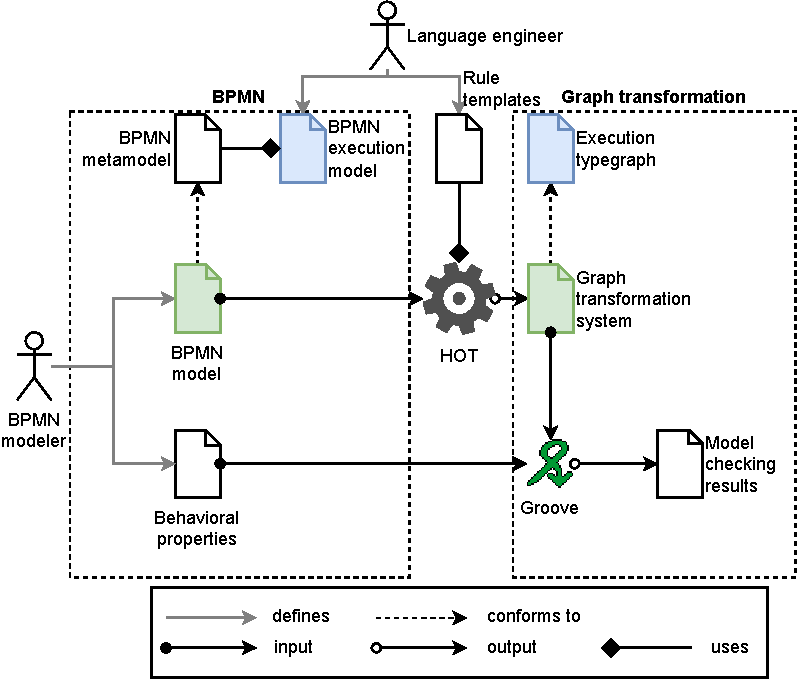
\includegraphics[width=0.8\textwidth]{images/bpmn_semantics-overview.pdf}
    \caption{Overview of the approach}
    \label{fig:approach}
\end{figure}

To begin the \gls*{bpmn} modeling process, a modeler first defines the \gls*{bpmn} model and its corresponding behavioral properties for evaluation.
This model must adhere to the \gls*{bpmn} metamodel as outlined in the \gls*{bpmn} specification by the Object Management Group \cite{objectmanagementgroupBusinessProcessModel2013}.
To create the state structure for BPMN, the \gls*{bpmn} execution metamodel is defined by language engineers, utilizing the \gls*{bpmn} metamodel as a foundation.
Typically, an execution metamodel is created by extending the structural \gls*{bpmn} metamodel.

Furthermore, we define a \gls*{hot} from \gls*{bpmn} models to \gls*{gt} systems.
We call the transformation \textit{higher-order} since the resulting graph-transformation systems represent model-transformations themselves \cite{tisiUseHigherOrderModel2009}.
The \gls*{hot} creates a \gls*{gt} system, i.e., \gls*{gt} rules and a start graph for a given \gls*{bpmn} model.
It is defined using rule generation templates, which describe how \gls*{gt} rules should be generated for each state-changing element in \gls*{bpmn} (see \autoref{sec:formalization}).
The obtained \gls*{gt} system conforms to the execution type graph which corresponds to the \gls*{bpmn} execution metamodel.
In the figure, we have colored both artifacts blue to visualize that they contain the same information.
Ultimately, we use Groove as an execution engine for the \gls*{gt} system and to check the behavioral properties that were defined earlier.

Our approach has been incorporated into a user-friendly, open-source web-based tool, which can be accessed without the need for installation.
The tool was validated using a comprehensive test suite.
Additionally, our approach is versatile as it can be applied to formalize other behavioral languages as well. 
To define the execution semantics of an alternate behavioral language, one simply needs to establish a new execution metamodel and \gls*{hot} (see the language engineer in \autoref{fig:approach}).


% Paper outline
The remainder of this paper is structured as follows.
First, in \autoref{sec:preliminaries}, we introduce \gls*{bpmn} and point out the theoretical background of this contribution.
Second, we describe the \gls*{bpmn} semantics formalization using the \gls*{hot} (\autoref{sec:formalization}) before explaining how this can be utilized for model checking general \gls*{bpmn} and custom properties (\autoref{sec:modelChecking}).
Then, in \autoref{sec:impl}, we present the web-based tool implementing our approach and benchmark the implementation.
Finally, we discuss related work regarding \gls*{bpmn} element coverage in \autoref{sec:relatedWork} and conclude in \autoref{sec:conclusion}.

\section{Preliminaries} \label{sec:preliminaries}

In this section, we will briefly introduce the execution semantics of BPMN, and readers are encouraged to consult \cite{freundRealLifeBPMNUsing2019} or the \gls*{bpmn} specification \cite{objectmanagementgroupBusinessProcessModel2013} for more in-depth information. 
Furthermore, our application of \gls*{gt}s to formalize the execution semantics of \gls*{bpmn} will be outlined in addition to a brief overview of the theoretical principles that underlie our use of \gls*{gt}s.



\subsection{BPMN}
\autoref{fig:bpmnMetamodel} depicts the structure of \gls*{bpmn} models with the corresponding concrete syntax \gls*{bpmn} symbols contained in clouds.

\begin{figure}[ht]
  \centering
  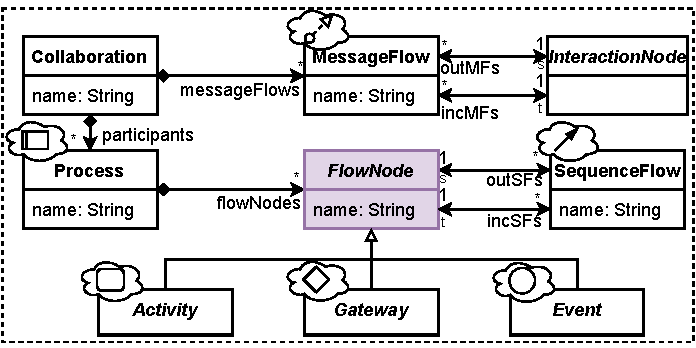
\includegraphics[width=0.7\linewidth]{images/bpmn_semantics-bpmn-metamodel.pdf}
  \caption{Excerpt of the \gls*{bpmn} metamodel \cite{objectmanagementgroupBusinessProcessModel2013}}
  \label{fig:bpmnMetamodel}
\end{figure}

A \gls*{bpmn} model is represented by a \textsf{Collaboration} that has \textsf{participants} and \textsf{MessageFlows} between \textsf{InteractionNodes}.
Each participant is a \textsf{Process} containing \textsf{FlowNodes} connected by \textsf{SequenceFlows}.
A \textsf{FlowNode} is either an \textsf{Activity}, \textsf{Gateway}, or \textsf{Event}.
Many types of \textsf{Activities}, \textsf{Gateways}, and \textsf{Events} exist.
Activities represent certain tasks to be carried out during a process, while events may happen during the execution of these tasks.
Furthermore, gateways model conditions, parallelizations, and synchronizations \cite{freundRealLifeBPMNUsing2019}.

The \gls*{bpmn} execution semantics is described using the concept of \textit{tokens} \cite{objectmanagementgroupBusinessProcessModel2013}, which can be located at sequence flows and specific flow nodes.
Tokens are consumed and created by flow nodes according to the connected sequence flows.
The \textsf{FlowNode} is colored purple in \autoref{fig:bpmnMetamodel} since it represents a state-changing element of \gls*{bpmn} as described in \autoref{sec:formalization}.

A \gls*{bpmn} process is triggered by one of its start events, leading to a token at each outgoing flow of the triggered start event.
% Activities
Activities can start when at least one token is on an incoming sequence flow.
The start of an activity will move the incoming token to the activity.
When an activity finishes, it deletes its token and adds one at each outgoing sequence flow.
% Gateways
Furthermore, different gateway types exist, such as parallelization, synchronization, XOR, and OR distribution of tokens.
% Events (basic)
Events delete and add tokens like activities but have additional semantics depending on their type.
For example, message events will add or delete messages.

\subsection{Theoretical background}
We use typed attributed graphs for the formalization of the \gls*{bpmn} execution semantics.
Each state, i.e., token distribution during the execution of a \gls*{bpmn} model, is represented as an attributed graph typed by the \gls*{bpmn} execution type graph, which we introduce in \autoref{sec:formalization}.

% Groove uses the single pushout approach with negative application conditions.
Regarding \gls*{gt}, we utilize the single-pushout (SPO) approach with negative application conditions (NAC) \cite{ehrigALGEBRAICAPPROACHESGRAPH1997}, as implemented in Groove \cite{rensinkGROOVESimulatorTool2004}.
In addition, we utilize \textit{nested rules} with quantification to make parts of a rule applied repeatedly or optionally \cite{rensinkNestedQuantificationGraph2006,rensinkHowMuchAre2017}.
Moreover, we utilize NACs to implement more intricate parts in the \gls*{bpmn} execution semantics, such as the termination of processes.


\section{BPMN semantics formalization} \label{sec:formalization}

The approach supports all the \gls*{bpmn} elements depicted in \autoref{fig:bpmnelementsOverview}.
These \gls*{bpmn} elements are divided into \textsf{Events}, \textsf{Gateways}, \textsf{Activities}, and \textsf{Edges}.
\textsf{Events} and \textsf{Activities} are further divided into subgroups.
Although all these elements have been implemented and tested (see \cite{krauterArtifactsICGT2023}), due to space limitations, we only explain the realization of the elements marked with a green background.
In the following, first we define the \gls*{bpmn} execution metamodel to represent the \gls*{bpmn} state structure, then we explain our formalization of the elements in \autoref{fig:bpmnelementsOverview}.


\begin{figure}[ht]
    \centering
    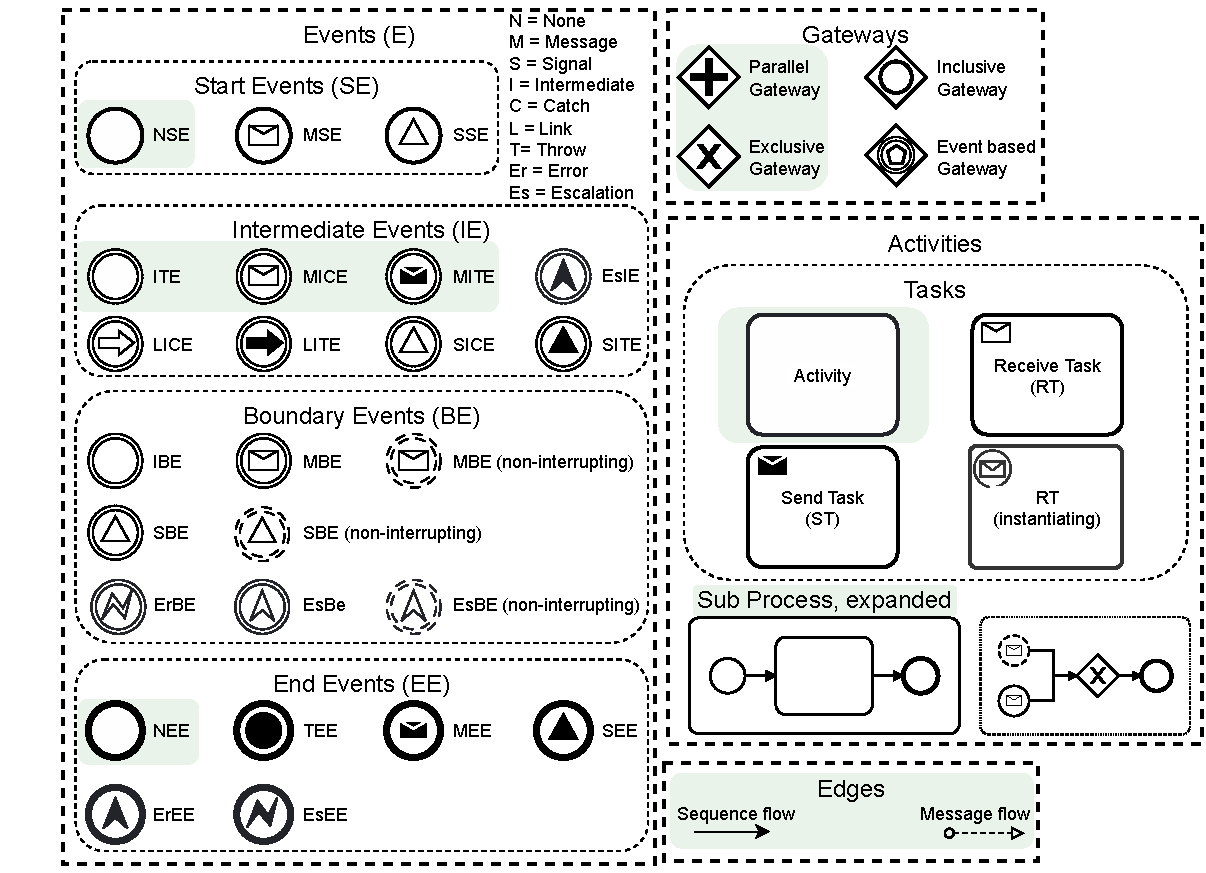
\includegraphics[width=0.99\textwidth]{images/bpmn_semantics-elements-overview.pdf}
    \caption{Overview of the supported \gls*{bpmn} elements (structure adapted from \cite{houhouFirstOrderLogicVerification2022})}
    \label{fig:bpmnelementsOverview}
\end{figure}


\subsection{BPMN execution metamodel}

In our formalization of BPMN, we utilize a token-based representation of the execution semantics, similar to the approach used in the informal description of the \gls*{bpmn} specification \cite{objectmanagementgroupBusinessProcessModel2013}.
To describe processes holding tokens during execution, we use the execution metamodel shown in \autoref{fig:typeGraph}, depicted as a UML class diagram.

\begin{figure}[ht]
  \centering
  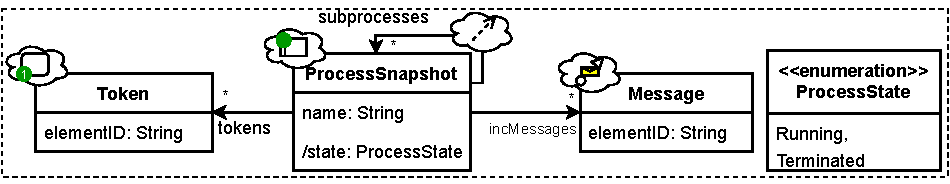
\includegraphics[width=0.6\linewidth]{images/bpmn_semantics-typegraph.pdf}
  \caption{BPMN execution metamodel}
  \label{fig:typeGraph}
\end{figure}

We use \textsf{ProcessSnapshot} to denote a running \gls*{bpmn} process with a specific token distribution that describes one state in the history of the process execution.
Every \textsf{ProcessSnapshot} has a set of \textsf{tokens}, incoming \textsf{messages}, and \textsf{subprocesses}.
A \textsf{ProcessSnapshot} has the state \textsf{Terminated} if it has no \textsf{tokens} or \textsf{subprocesses}.
Otherwise, it has the state \textsf{Running}.
A \textsf{Token} has an \textsf{elementID}, which points to the \gls*{bpmn} \textsf{Activity} or the \textsf{SequenceFlow} at which it is located.
A \textsf{Message} has an \textsf{elementID} pointing to a \textsf{MessageFlow}.
To concisely depict graphs conforming to this type graph, we introduce a concrete syntax in the clouds attached to the elements.
Our concrete syntax extends the \gls*{bpmn} syntax by adding process snapshots, subprocess relations, tokens, and messages.
Tokens are represented as colored circles drawn at their specified positions in a model.
In addition, we use colored circles at the top left of the bounding box, representing instances of the \gls*{bpmn} \textsf{Process}; these circles represent process snapshots.
The token's color must match the color of the process snapshot holding the token.
The concrete syntax was inspired by the bpmn-js-token-simulation \cite{camundaservicesgmbhBpmnjsTokenSimulation2023}.


The execution metamodel is a UML class diagram without operations, which can be seen as an attributed type graph \cite{heckelGraphTransformationSoftware2020}.
Using execution metamodel as the type graph, we can now define how the start graph and graph-transformation rules for the different \gls*{bpmn} elements are created.

Since our approach is based on a \gls*{hot} from \gls*{bpmn} to \gls*{gt} systems, we generate a \textit{start graph} and \textit{\gls*{gt} rules} for each given \gls*{bpmn} model.
Generating the start graph for a \gls*{bpmn} model is straightforward.
First, for each process in the \gls*{bpmn} model, we generate a process snapshot if the process contains a none start event (NSE).
An NSE describes a start event without a trigger (none).
Then, for each NSE we add one token to each outgoing sequence flow.
An example of a start graph is shown in \autoref{fig:startGraph} using abstract and concrete syntax.

\begin{figure}[ht]
    \centering
    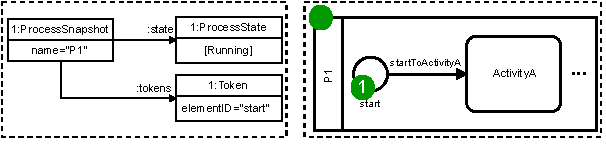
\includegraphics[width=0.85\textwidth]{images/startGraph.pdf}
    \caption{Example start graph in abstract (left) and concrete syntax (right)}
    \label{fig:startGraph}
\end{figure}

The \gls*{hot} generates one or more \gls*{gt} rules for each \textsf{FlowNode}, i.e., state-changing element in a \gls*{bpmn} model.
In order to provide a better understanding of the transformation process, we will begin by presenting two example results, namely the generated rules for an activity (as shown in \autoref{fig:bpmnelementsOverview}).
Following this, we will delve into an explanation of how our \gls*{hot} creates these rules as well as others.

\autoref{fig:gtRuleAbstract} depicts an example \gls*{gt} rule ($L \to R$) to start an activity in abstract syntax.
The rule is straightforward, moving a token from the incoming sequence flow to the activity itself.
For the rest of the paper, we will depict all rules in the concrete syntax introduced earlier.
The rule from \autoref{fig:gtRuleAbstract} depicted in concrete syntax is shown on the left in \autoref{fig:gtRuleConcrete}.
The rule on the right in \autoref{fig:gtRuleConcrete} implements the termination of an activity, which will move one token from the activity to the outgoing sequence flow.

\begin{figure}[ht]
    \centering
  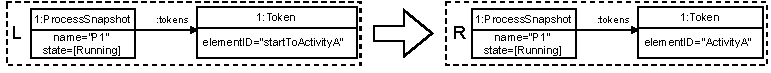
\includegraphics[width=1\textwidth]{images/rule_abstract.pdf}
  \caption{Example \gls*{gt} rule to start an activity (abstract syntax)}  \label{fig:gtRuleAbstract}
\end{figure}


\begin{figure}[ht]
    \centering
  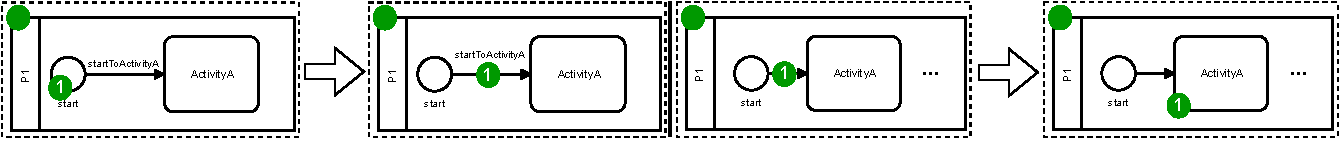
\includegraphics[width=1\textwidth]{images/rule_concrete.pdf}
  \caption{Example \gls*{gt} rule to start (left) and terminate (right) an activity}
  \label{fig:gtRuleConcrete}
\end{figure}

To summarize, we described two example rules and introduced a concrete syntax to depict them concisely and understandably.
In the following subsections, we use this concrete syntax to describe how these rules and rules for other flow nodes are generated by our \gls*{hot}.
Elements of the \gls*{hot} are depicted using rule generation templates that describe how specific rules are created for various flow nodes.

\subsection{Process instantiation and termination} \label{subsec:instAndTermination}

Start events do not need \gls*{gt} rules since the generated start graph of the \gls*{gt} system will contain a token for each outgoing sequence flow of a NSE.
Other types of start events are triggered in corresponding throw event rules.

\autoref{fig:startAndEndTemplate} depicts the rule generation template for end events (\textsf{NEE} in \autoref{fig:bpmnelementsOverview}).
All rule generation templates show a state-changing element (\textsf{FlowNode}) with surrounding flows in the left column and the applicable rule generation in the right column.
The left column shows instances of the \gls*{bpmn} metamodel (\autoref{fig:bpmnMetamodel}), and the right column shows the generated rules typed by the \gls*{bpmn} execution metamodel (see \autoref{fig:typeGraph}).
If more than one rule is generated from a \textsf{FlowNode}, an expression defines how each rule is generated.
For example, the expression $\forall \text{sf} \in \text{E.incSFs}$ for the rule generation template of end events (see \autoref{fig:startAndEndTemplate}) generates one rule for each incoming sequence flow \textit{sf} of the end event \textit{E}.
We use ``.'' in expressions to navigate along the associations of the \gls*{bpmn} metamodel shown in \autoref{fig:bpmnMetamodel}.
In the example, \textsf{E.incSFs} means following all \textsf{incSFs} links for a \textsf{FlowNode} object, resulting in a set of \textsf{SequenceFlow} objects.

\begin{figure}[ht]
    \centering
    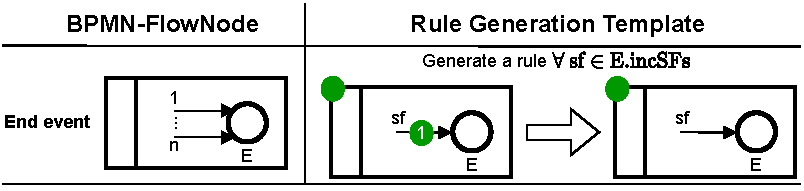
\includegraphics[width=.8\textwidth]{images/end_template.pdf}
    \caption{Rule generation templates for start and end events}
    \label{fig:startAndEndTemplate}
\end{figure}
    
% End Event
The generated end event rules delete tokens one by one for each incoming sequence flow.
However, they do not terminate processes.
% General termination rule
Process termination is implemented with a generic rule---independent of the input \gls*{bpmn} model---which is applicable to all process snapshots.
The termination rule in \autoref{fig:terminationRule} is automatically generated once during the \gls*{hot}.
The rule changes the state of the process snapshot from running to terminated if it has neither tokens nor subprocesses.

\begin{figure}[ht]
    \centering
    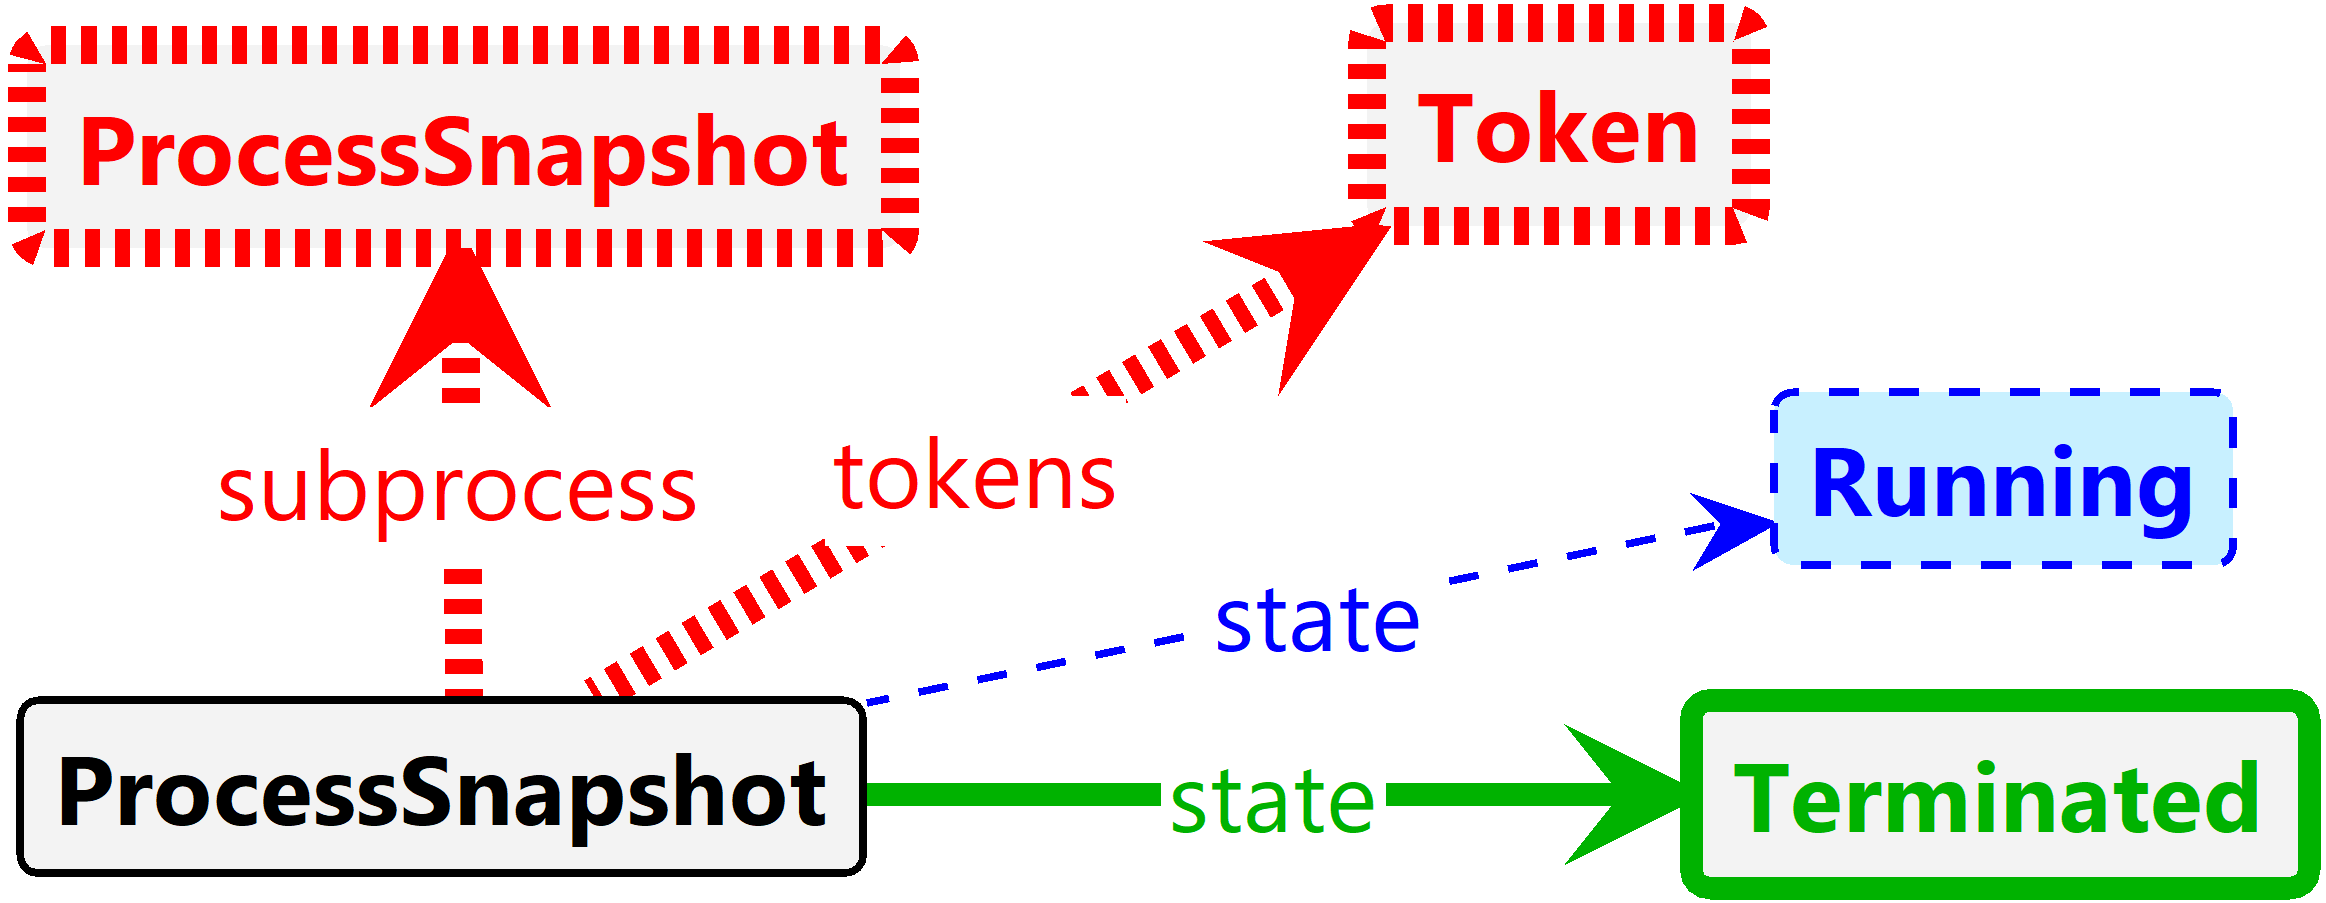
\includegraphics[width=.5\textwidth]{images/terminate_groove.png}
    \caption{Termination rule in Groove}
    \label{fig:terminationRule}
\end{figure}

\subsection{Activities \& Subprocesses}

% Normal activities
\autoref{fig:activityTemplates} depicts the rule generation templates for activities and subprocesses (see \autoref{fig:bpmnelementsOverview}).
Activity execution is divided into two steps implemented by two rule templates.
The first template generates one rule for each incoming sequence flow to start the activity.
An activity can be started using a token positioned at any of its incoming sequence flows.
This rule template generates the sample rule in the right of \autoref{fig:gtRuleConcrete}.
Having multiple incoming or outgoing sequence flows for a flow node is considered bad practice since the implicitly encoded gateways should be explicit to avoid confusion.
Our formalization still supports this behavior, but we recommend using static analyzers to avoid such models \cite{camundaservicesgmbhBpmnlint2023}.

The second template generates one rule that terminates the activity.
It deletes a token at the activity and adds one at each outgoing sequence flow.
This implicitly encodes a parallel gateway (see \autoref{fig:gatewayTemplates}) but should be avoided as described earlier. 

\begin{figure}[ht]
    \centering
    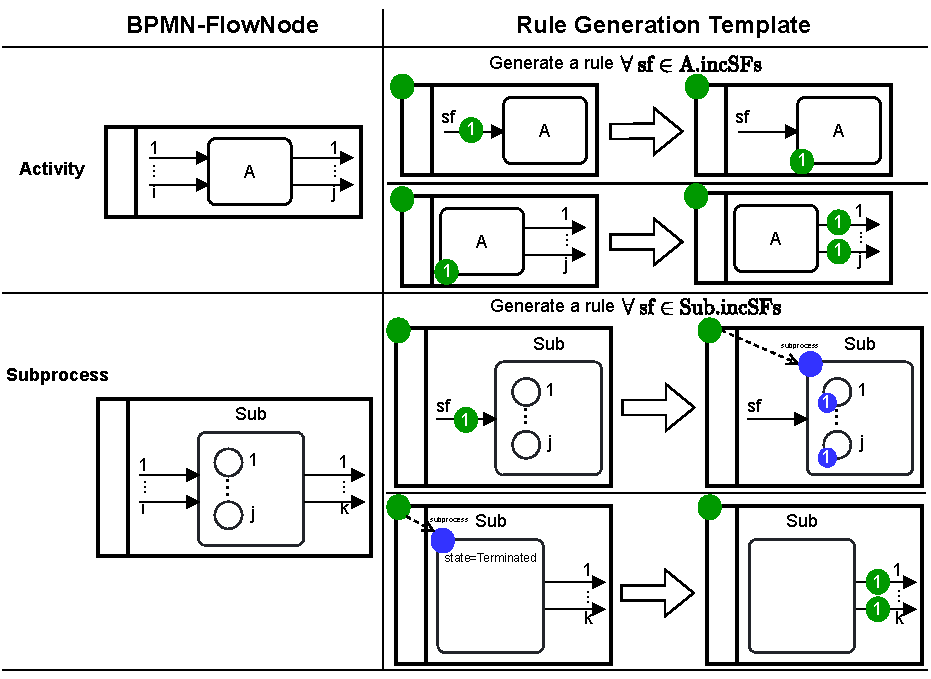
\includegraphics[width=1\textwidth]{images/activities_template.pdf}
    \caption{Rule generation template for activities and subprocesses}
    \label{fig:activityTemplates}
\end{figure}

% Subprocesses/Call activities
Subprocess execution is like activity execution.
The upper part of the template generates one rule for each incoming sequence flow.
The rule deletes an incoming token and adds a process snapshot representing a subprocess. 
The created process snapshot is represented with a colored circle on the top left corner of the subprocess with a token at each outgoing sequence flow of its start events (similar to start graph generation).
There is a \textit{subprocess} link between the process snapshots to depict the \textsf{subprocesses} relation in \autoref{fig:typeGraph}.
If the subprocess has no start events, a token will be added to every activity and gateway with no incoming sequence flows.

The bottom part of the template generates one rule to delete a terminated process snapshot and adds tokens at each outgoing sequence flow.
Subprocesses are terminated by the termination rule (see section \ref{subsec:instAndTermination}).


% Send/Receive tasks (mentioned/shown with message events later)
\subsection{Gateways}
\autoref{fig:gatewayTemplates} depicts the rule generation templates for parallel and exclusive gateways (see \autoref{fig:bpmnelementsOverview}).
A parallel gateway can synchronize and fork the control flow simultaneously.
Thus, one rule is generated that deletes one token from each incoming sequence flow and adds one token to each outgoing sequence flow.

\begin{figure}[ht]
    \centering
    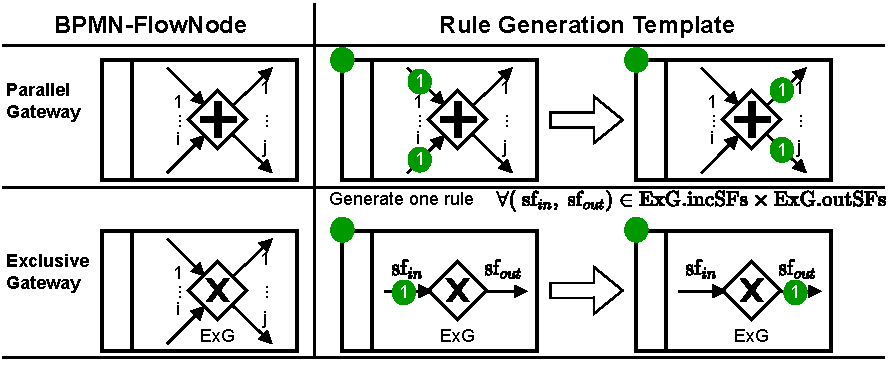
\includegraphics[width=1\textwidth]{images/gateways_template.pdf}
    \caption{Rule generation template for gateways}
    \label{fig:gatewayTemplates}
\end{figure}

Exclusive Gateways are triggered by exactly one incoming sequence flow, and exactly one outgoing sequence flow will be triggered as a result.
Thus, one rule must be generated for every combination of incoming and outgoing sequence flows.
However, the resulting rule is simple since it only deletes a token from an incoming sequence flow and adds one to an outgoing sequence flow.

\subsection{Message Events}
% MITE
\autoref{fig:messageEventTemplates} depicts the rule generation templates for \textit{message intermediate throw events} and \textit{message intermediate catch events} (\textsf{MITE} and \textsf{MICE} in \autoref{fig:bpmnelementsOverview}).
% Message throw with intermediate catch message events
The first rule template describes how MITEs interact with MICEs.
A MITE deletes an incoming token and adds one at each outgoing sequence flow.
In addition, it sends one message to each process by adding it to the incoming messages of the process.
However, sending each message is optional, meaning that if a process is not ready to consume a message immediately, the message is not added.
A process can consume a message if its MICE has at least one token at an incoming sequence flow (see \autoref{fig:messageEventTemplates}).
We implement optional message sending using nested rules with quantification.
Concretely, we use an optional existential quantifier \cite{rensinkNestedQuantificationGraph2006} (see blue dotted rectangle marked with optional in \autoref{fig:messageEventTemplates}) to send a message only if the receiving process is ready to consume it.

\begin{figure}[ht]
    \centering
    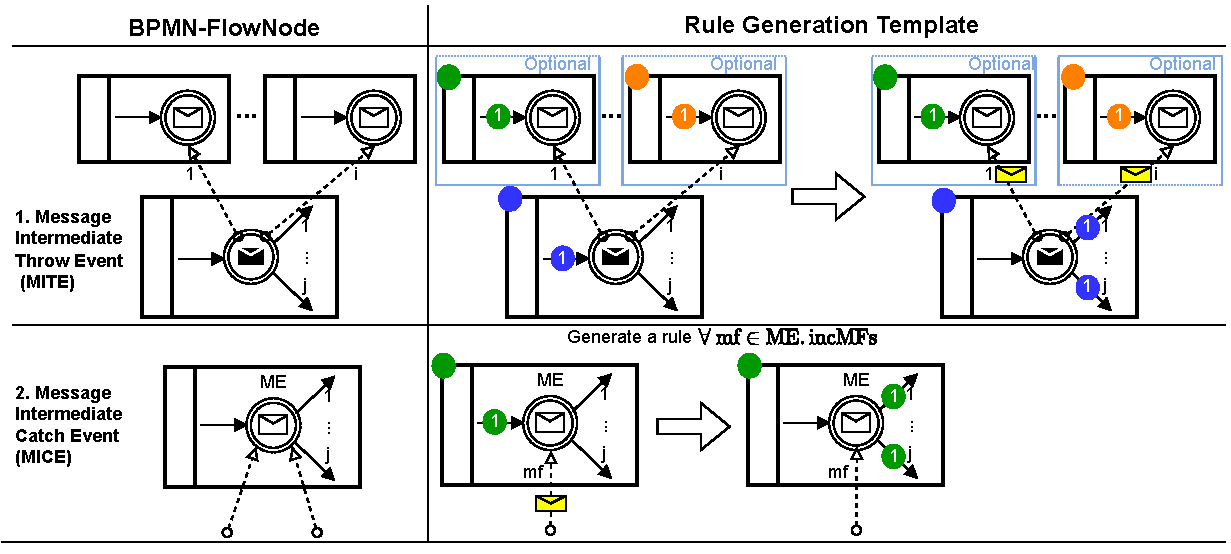
\includegraphics[width=1\textwidth]{images/bpmn_semantics-message_templates.pdf}
    \caption{Rule generation templates for message events}
    \label{fig:messageEventTemplates}
\end{figure}

% MICE
The second rule template in \autoref{fig:messageEventTemplates} shows the behavior of MICEs.
To trigger a MICE, only one message at an incoming \textit{message flow} is needed.
Thus, one rule is generated for each incoming \textit{message flow}.
The rule template shows that MICEs delete one message and one token, as well as add a token at each outgoing sequence flow.


\section{Model checking BPMN} \label{sec:modelChecking}

Model checking---and verification in general---of \gls*{bpmn} models is necessary to ensure the correctness and reliability of business processes, which ultimately leads to increased efficiency, reduced costs, and improved user satisfaction.
Using our approach, model checking a \gls*{bpmn} model is possible using the generated \gls*{gt} system and a set of temporal properties with atomic propositions.
Properties are defined using a temporal logic, such as CTL and LTL.
In this paper we will use CTL.
An atomic proposition is formalized as a graph and holds in a given state if a match exists from the graph representing the proposition to the graph representing the state \cite{kastenbergModelCheckingDynamic2006}.

We differentiate between \textit{general \gls*{bpmn} properties} defined for all \gls*{bpmn} models and \textit{custom properties} tailored towards a particular \gls*{bpmn} model.
We do not consider structural properties (like conformance to the syntax of BPMN) since they can be checked using a standard modeling tool without implementing execution semantics.
We will now give an example of two predefined general \gls*{bpmn} properties and show how they can be checked using our approach.
Then, we describe how custom properties can be defined and checked.

\subsection{General BPMN properties}
\textit{Safeness} and \textit{Soundness} properties are defined for \gls*{bpmn} in \cite{corradiniClassificationBPMNCollaborations2018}.
A \gls*{bpmn} model is \textit{safe} if, during its execution, at most one token occurs along the same sequence flow \cite{corradiniClassificationBPMNCollaborations2018}.
Soundness is further decomposed into (i) \textit{Option to complete}: any running process instance must eventually complete, (ii) \textit{Proper completion}: after completion, each token of the process instance must be consumed by a different end event, as well as (iii) \textit{No dead activities}: each activity can be executed in at least one process instance \cite{corradiniClassificationBPMNCollaborations2018}.
In the following, we will describe how to implement the \textit{Safeness} and \textit{Option to complete} properties.

% Safeness
We specify \textit{Safeness} as the CTL property defined in \eqref{eq:safeness}.
The atomic property \textsf{Unsafe} is true if two tokens of one process snapshot point to the same sequence flow.
It is shown in \autoref{fig:unsafe}.

\begin{figure}[ht]
    \centering
    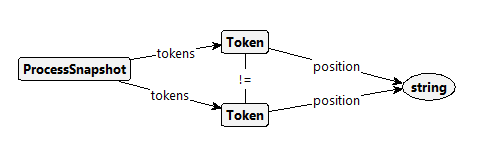
\includegraphics[width=0.7\textwidth]{images/Unsafe.png}
    \caption{The atomic proposition \textit{Unsafe} in Groove.}
    \label{fig:unsafe}
\end{figure}

% Option to complete
\textit{Option to complete} is specified using the CTL property defined in \eqref{eq:optionToComplete}.
The atomic proposition \textsf{AllTerminated} is true if there exists no process snapshot in the state \textsf{Running}, i.e., all process snapshots are \textsf{Terminated}.
\textsf{AllTerminated} is given in \cite{krauterArtifactsICGT2023}.

\noindent\begin{minipage}{.5\linewidth}
\begin{equation} \label{eq:safeness}
  AG(\neg \,\text{Unsafe})
\end{equation}
\end{minipage}%
\begin{minipage}{.5\linewidth}
\begin{equation} \label{eq:optionToComplete}
  AF(\text{AllTerminated}) 
\end{equation}
\end{minipage}
\vskip.3\baselineskip

Checking the properties \textit{Safeness}, \textit{Option to Complete}, and \textit{No Dead Activities} is implemented in our tool \cite{krauterArtifactsICGT2023}.
The property \textit{Proper Completion} is not yet implemented, but all the information needed can be found in the \gls*{gt} systems state space.

\subsection{Custom properties} \label{subsec:customProperties}
% Defining atomic propositions in BPMN is a novelty.
To make model checking user-friendly, we envision modelers defining atomic propositions in the extended \gls*{bpmn} syntax, i.e., the concrete syntax introduced in \autoref{fig:typeGraph}.
Therefore, to define an atomic proposition, a modeler adds process snapshots and tokens to a \gls*{bpmn} model, which we can automatically convert to a graph representing an atomic proposition.

For example, the token distribution shown in \autoref{fig:atomicProposition} defines two running process snapshots with a token at activity A.
Differently colored tokens define different process snapshots.
A modeler could use this atomic proposition, for example, to check if, eventually, two processes are executing activity A simultaneously by creating an LTL/CTL property.
Thus, a modeler does not need to know the \gls*{gt} semantics used for execution.

However, the modeler must still know the temporal logic, such as LTL and CTL, to express his properties.
In the future, a domain-specific property language for \gls*{bpmn} would further lessen the amount of knowledge required from the modeler \cite{meyersProMoBoxFrameworkGenerating2014}. 


\begin{figure}[ht]
    \centering
    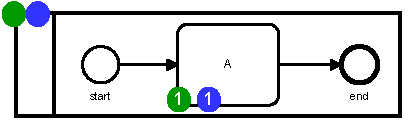
\includegraphics[width=0.45\textwidth]{images/bpmn_semantics-atomic-proposition.pdf}
    \caption{Token distribution defining an atomic proposition.}
    \label{fig:atomicProposition}
\end{figure}


\section{Implementation} \label{sec:impl}
In this section, we will present our tool and then describe experiments regarding its performance.

\subsection{BPMN Analyzer tool}

Our approach is implemented in a web-based tool called \textit{BPMN Analyzer} that is open-source, publicly available, and does not require any installation \cite{krauterArtifactsICGT2023}.
\autoref{fig:implScreenshot} depicts a screenshot of BPMN Analyzer.

The modeler can create or upload a \gls*{bpmn} model, which can then be verified using either \gls*{bpmn}-specific properties or custom CTL properties in the verification section.
BPMN Analyzer can generate a \gls*{gt} system for the supplied \gls*{bpmn} model and run model checking in Groove \cite{kastenbergModelCheckingDynamic2006}. 
To evaluate the correctness of our \gls*{hot}, we have created a comprehensive test suite that verifies the correct generation of rules for the implemented \gls*{bpmn} elements \cite{krauterArtifactsICGT2023}.
Additionally, we have conducted a performance benchmark for our approach, as described in the next section.


% Use impl/impl_short/impl_very_short
\begin{figure}[ht]
    \centering
    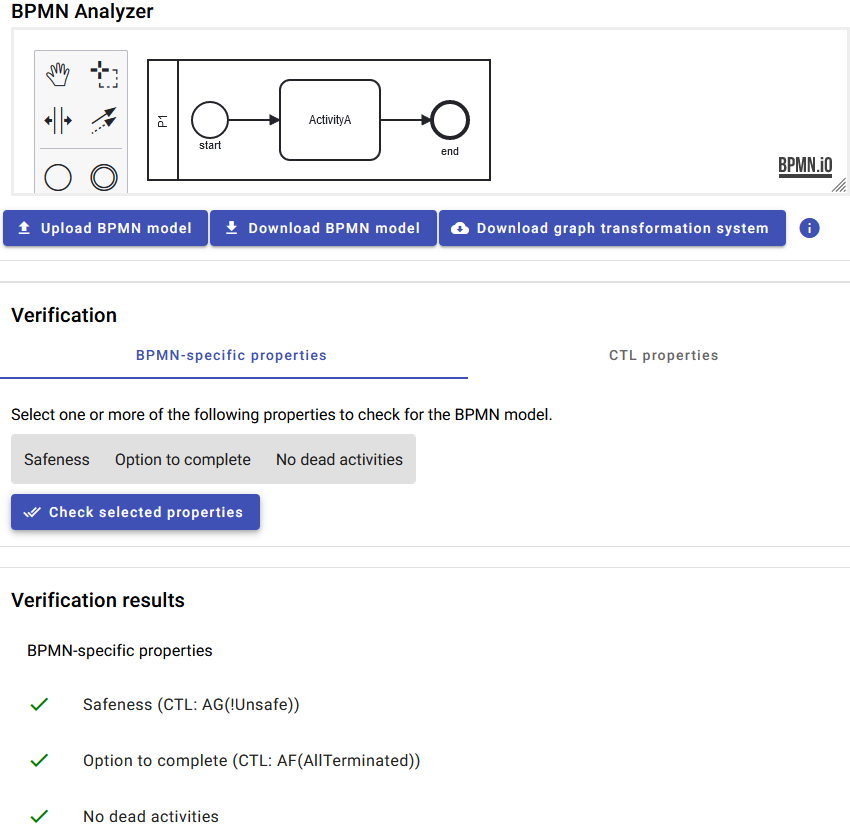
\includegraphics[width=0.7\textwidth]{images/impl_short.png}
    \caption{Screenshot of the BPMN Analyzer tool}
    \label{fig:implScreenshot}
\end{figure}

\subsection{Experiments}

Model checking is a useful technique but often falls short in practice due to insufficient performance.
Poor performance might have many reasons, most notably large models leading to state space explosion.
We experimented with ten different \gls*{bpmn} models from \cite{houhouFirstOrderLogicVerification2022} to assess the performance of our implementation.
We picked the models at random besides disregarding some models that were similar.
The models include realistic business process models (001, 002, and 020) \cite{houhouFirstOrderLogicVerification2022}.

To calculate the average runtime, we used the hyperfine benchmarking tool \cite{peterHyperfine2022} (version 1.15.0), which ran state space exploration for each \gls*{bpmn} model ten times.
The experiment was run on Windows 11 (AMD Ryzen 7700X processor, 32 GB RAM) using Groove version 5.8.1 \cite{krauterArtifactsICGT2023}. 

First, we ran our \gls*{hot} for the \gls*{bpmn} models.
The \gls*{hot} took less than one second to generate a \gls*{gt} system for each model.
Thus, the generation of the \gls*{gt} systems is fast enough.
Furthermore, we estimate most of the time is spent writing the \gls*{gt} system to disk.

Second, we ran a full state exploration using the resulting ten \gls*{gt} systems, see \autoref{table:stateSpaceBenchmark}.
The exploration takes roughly one second for most of the models.
Only model \textit{020} needs nearly two seconds due to its larger state space.
Furthermore, we estimate that up to one second is spent before state space exploration, most likely reading the \gls*{gt} system files.
For example, Groove reports only 722 ms for state space exploration for model \textit{020}.

We conclude that our approach is sufficiently fast for models of normal size.
In addition, there is still room for optimization, such as avoiding costly I/O to disk.
A comprehensive benchmark, including a detailed comparison to other tools, is left for future work.

\begin{table}[ht]
\centering

\begin{tabular}{| c | c | c || c | c | c |}
 \hline
 BPMN model & Processes & Nodes (gw.) & States & Transitions & Total time \\
 \hline\hline
 001 & 2 & 17(2) & 68 & 118 & $\sim$ 1.00 s \\
 \hline
 002 & 2 & 16(2) & 62 & 108 & $\sim$ 0.97 s \\
 \hline
 007 & 1 & 8(2) & 45 & 81 & $\sim$ 0.92 s \\
 \hline
 008 & 1 & 11(2) & 49 & 85 & $\sim$ 0.93 s \\
 \hline
 009 & 1 & 12(2) & 137 & 308 & $\sim$ 1.01 s \\
 \hline
 010 & 1 & 15(2) & 162 & 357 & $\sim$ 1.04 s \\
 \hline
 011 & 1 & 15(2) & 44 & 69 & $\sim$ 0.97 s \\
 \hline
 015 & 1 & 14(2) & 53 & 86 & $\sim$ 0.95 s \\
 \hline
 016 & 1 & 14(2) & 44 & 68 & $\sim$ 0.94 s \\
 \hline
 020 & 1 & 39(6) & 3060 & 8584 & $\sim$ 1.75 s \\
 \hline
\end{tabular}
\caption[Experimental results for a full state space exploration in Groove]{Experimental results for a full state space exploration in Groove}
\label{table:stateSpaceBenchmark}
\end{table}

\section{Related work} \label{sec:relatedWork}
% Van gorp
A \gls*{bpmn} formalization based on in-place \gls*{gt} rules is given in \cite{vangorpVisualTokenbasedFormalization2013}.
The formalization covers a substantial part of the \gls*{bpmn} specification, including complex concepts such as inclusive gateways and compensation.
In addition, the \gls*{gt} rules are visual and thus can be aligned with the informal description of the execution semantics of BPMN.
A key difference to our approach is that the rules in \cite{vangorpVisualTokenbasedFormalization2013} are general and can be applied to every \gls*{bpmn} model, while we generate specific rules for each \gls*{bpmn} model using our \gls*{hot}.
Thus, our approach can be seen as a program specialization compared to \cite{vangorpVisualTokenbasedFormalization2013} since we process a concrete \gls*{bpmn} model before its execution.
However, they do \textit{not} support property checking since their goal is only formalization.

% BProve/Corradini
The tool \textit{BProVe} is based on formal \gls*{bpmn} semantics given in rewriting logic and implemented in the Maude system \cite{corradiniFormalApproachAnalysis2021}.
Using this formal semantics, they can verify custom LTL properties and general \gls*{bpmn} properties, such as Safeness and Soundness.

% fbpmn/Houhou
The verification framework \textsf{fbpmn} uses first-order logic to formalize and check \gls*{bpmn} models \cite{houhouFirstOrderLogicVerification2022}.
This formalization is then realized in the TLA\textsuperscript{+} formal language and can be model-checked using TLC.
Like BProVe, \textsf{fbpmn} allows checking general \gls*{bpmn} properties, such as Safeness and Soundness.
Furthermore, they focus on different communication models besides the standard in the \gls*{bpmn} specification and support time-related constructs.
We currently disregard time-related constructs \cite{duranVerifyingTimedBPMN2017,houhouFirstOrderLogicVerification2022} and data flow \cite{corradiniFormalisingAnimatingMultiple2022,el-saberCMMICMComplianceChecking2015}.

\autoref{tab:supportedelements} shows which \gls*{bpmn} elements are supported by the approaches mentioned above compared to ours.
The coverage of \gls*{bpmn} elements greatly impacts how useful each approach is in practice.
% Summarize the findings and explain them in more detail
Our approach covers most of the \gls*{bpmn} elements compared to other current approaches.
In addition, it covers the most important elements found in practice since we come close to the element coverage of popular process engines such as Camunda \cite{camundaservicesgmbhBPMNImplementationReference2023}.

\begin{table}[htbp]
    \caption{\gls*{bpmn} elements supported by different formalizations (based on \cite{vangorpVisualTokenbasedFormalization2013}).}
    \label{tab:supportedelements}
    \begin{threeparttable}
    \begin{tabular}{l l l l l}
    \hline
      \gls*{bpmn} element/feature & Van Gorp &  Corradini & Houhou & This\\
      & et al. \cite{vangorpVisualTokenbasedFormalization2013} & et al. \cite{corradiniFormalApproachAnalysis2021}& et al. \cite{houhouFirstOrderLogicVerification2022} & paper\\
      \hline
      \textit{Instantiation and termination} & &\\
      Start event instantiation & X & X & X & X\\
      Exclusive event-based gateway instantiation & X & & & X\\
      Parallel event-based gateway instantiation &  & & & \\
      Receive task instantiation & & & & X\\
      Normal process completion & X & X & X & X\\
      \textit{Activities} & & & &\\
      Activity & X & X & X & X\\
      Subprocess & X & & X & X\\
      Ad-hoc subprocesses & & & &\\
      Loop activity & X & & &\\
      Multiple instance activity & & & & \\
      \textit{Gateways} & & & &\\
      Parallel gateway & X & X & X & X\\
      Exclusive gateway & X & X & X & X\\
      Inclusive gateway (split) & X & X & X & X\\
      Inclusive gateway (merge) & X & & X & X\\
      Event-based gateway &  & X\tnote{1} & X & X\\ % No timer and conditional events after event based gateway supported.
      Complex gateway & & & &\\
      \textit{Events} & & & & \\
      None Events & X & X & X & X\\
      Message events & X & X & X & X\\
      Timer Events & & & X & \\
      Escalation Events & & & & X\\
      Error Events & X & & & X\\
      Cancel Events & X & & &\\
      Compensation Events & X & & &\\
      Conditional Events & & & &\\
      Link Events & X & & & X\\
      Signal Events & X & & & X\\
      Multiple Events &  & & & \\
      Terminate Events & X & X & X & X\\
     Boundary Events & X\tnote{2} & & X\tnote{3} & X\\ % To the same extent as the event support
      Event subprocess &  &  &  & X\\
    \end{tabular}
    \begin{tablenotes}
        \item[1] Does not support receive tasks after event-based gateways.
        \item[2] Only supports interrupting boundary events on tasks, not subprocesses.
        \item[3] Only supports message and timer events.
    \end{tablenotes}
    \end{threeparttable}
\end{table}


\section{Conclusion \& future work} \label{sec:conclusion}
This paper makes two main practical contributions.
First, we conceptualize a new approach utilizing a \gls*{hot} to formalize the semantics of behavioral languages.
Our approach moves complexity from the \gls*{gt} rules to the rule templates making up the \gls*{hot}.
Furthermore, the approach can be applied to any behavioral language if one can define its \textit{state structure} and identify its \textit{state-changing elements}.

Second, we apply our approach to BPMN, resulting in a comprehensive formalization regarding element coverage (compared to the literature and industrial process engines) that supports checking behavioral properties.
Furthermore, our contribution is implemented in an open-source web-based tool to make our ideas easily accessible to other researchers and practitioners.

Future work targets both of our main contributions.
First, we plan a detailed comparison of our \gls*{hot} approach with approaches that utilize fixed rules.
It will be interesting to investigate how the two approaches differ, for example, in runtime during state space generation.
Second, we aim to improve our formalization and the resulting tool in multiple ways.
We intend to extend our formalization to support the remaining few \gls*{bpmn} elements used in practice and want to turn the modeling environment of our tool into an interactive simulation environment.
In addition, we can use this environment to visualize potential counterexamples in cases where behavioral properties are violated.

\bibliographystyle{splncs04} 
\bibliography{bib}

% The appendix is not published.
% I added it to showcase the tool's capabilities in more detail.
\section{Appendix}


This section shows examples of our tool checking general \gls*{bpmn} properties.
Our tool and the example models are available as artifacts \cite{krauterArtifactsICGT2023}.

\subsection{Safeness example}
\autoref{fig:unsafeSample} shows a screenshot of the tool detecting an unsafe situation.
Unfortunately, Groove does not provide a counterexample when running CTL model checking through the console.
Thus, we cannot highlight where the model is unsafe.
In this case, the sequence flow \textit{Unsafe} is unsafe.

The exclusive gateway merges the sequence flows but does not synchronize.
Thus, the outgoing sequence flow can hold two tokens, and Activity C is executed twice, which might not be intended.
This could be a simple mistake of picking an exclusive instead of a parallel gateway.

\begin{figure}[ht]
    \centering
    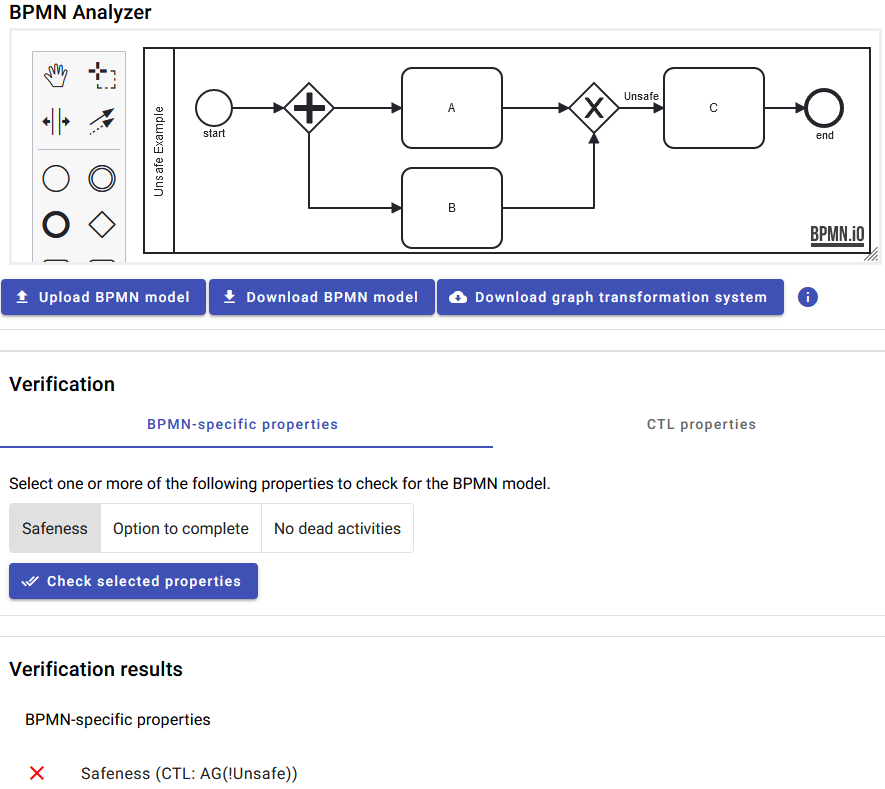
\includegraphics[width=1\textwidth]{artifacts/appendix/unsafe_sample.png}
    \caption{Screenshot of the tool detecting an unsafe situation}
    \label{fig:unsafeSample}
\end{figure}

\subsection{Option to complete example}
\autoref{fig:optionToCompleteSample} shows a screenshot of the tool checking the \textit{Option to complete} property.

\textit{Option to complete} does not hold for the BPMN model since the scan (second exclusive gateway) might never be successful.
This leads to an infinite loop.
Thus, not every process might terminate.

\begin{figure}[ht]
    \centering
    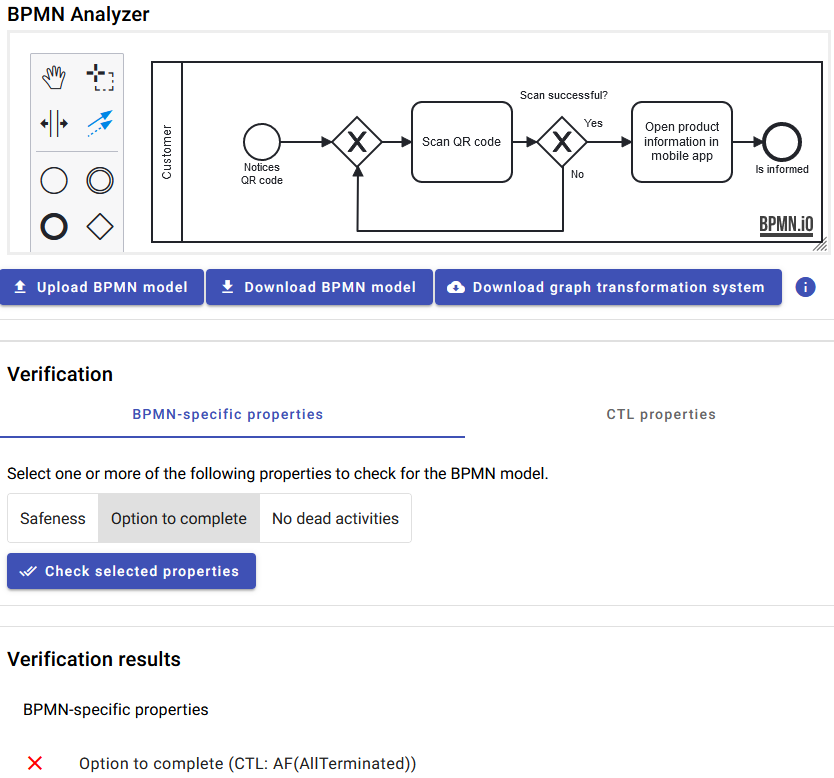
\includegraphics[width=1\textwidth]{artifacts/appendix/option_to_complete_sample.png}
    \caption{Screenshot of the tool checking \textit{Option to complete}}
    \label{fig:optionToCompleteSample}
\end{figure}

\subsection{No dead activities example}
\autoref{fig:deadSample} shows a screenshot of the tool detecting a dead activity.
Activity C is \textit{dead}, which is highlighted when checking for dead activities.

\begin{figure}[ht]
    \centering
    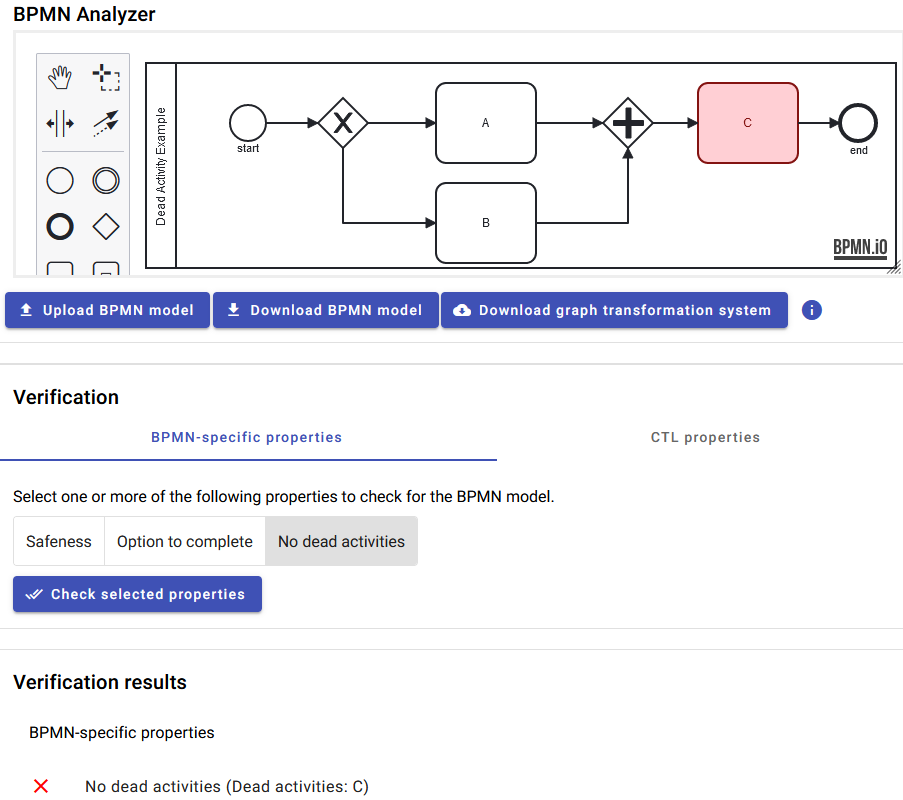
\includegraphics[width=1\textwidth]{artifacts/appendix/dead_sample.png}
    \caption{Screenshot of the tool detecting a dead activity}
    \label{fig:deadSample}
\end{figure}

The parallel gateway is incorrect since it cannot synchronize two sequence flows that never split.
The mistake can be fixed by using one gateway type consistently.
However, in practice, erroneous situations might be much more complex when multiple processes communicate using messages, signals, and other events.

\end{document}
